\subtitle{Terreno urbano e industrial}
 \begin{frame}{}
     \maketitle
 \end{frame}
 
 \begin{frame}{Terreno Urbano/Industrial}
     
     
 \end{frame}
 
 \begin{frame}{Flujo alrededor de obstaculos}
 
 Depende de la altura de los obstaculos ($H_r$) y de el espaciado entre ellos ($S_r$). En menor medida también depende del ancho de los obstaculos.
 
 \begin{figure}
     \centering
     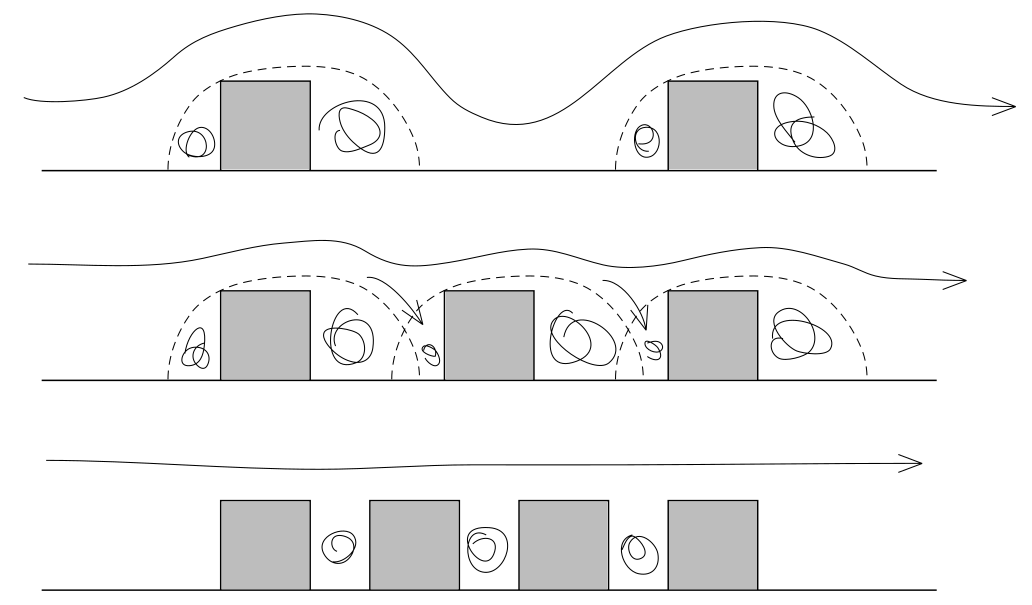
\includegraphics[width=0.6\textwidth]{img/flow_above_obstacles.png}
     \caption{Regimenes de flujo sobre terrano urbano. Isolated roughness flow si $S_r/H_r > 3$ (arriba). $3>S_r/H_r> 1.5$ wake interference flow (medio), $S_r/H_r<1.5$ skimming flow (abajo).}
 \end{figure}
 \end{frame}
 
 \begin{frame}{Rugosidad cerca de la superficie}
     
     
 \end{frame}

 \begin{frame}{Perfil de vientos cerca de la superficie}
     
     
 \end{frame}
 
 \begin{frame}{Turbulencia cerca de la superficie}
     
     
 \end{frame}